\chapter{Milestone 4}
\section{Force-Derivation from the Lenard Jones Potential}

\begin{comment}
1. Put the python code here
2. write the base equations (lj + f)
3. write the result form the python code 
4. write some text
5. c++ code that results from this?
\end{comment}
%% equations
\begin{equation}
	\overrightarrow{f_{k}} = \sum_{i}^{}\frac{\partial V}{\partial r_{ik}} \hat{r_{ik}}
\end{equation}

\begin{equation}
	V(r) = 4\epsilon\bigg[\Big(\frac{\sigma}{r}\Big)^{12}- \Big(\frac{\sigma}{r}\Big)^{6} \bigg]
\end{equation}

\begin{equation}
	\frac{\partial V}{\partial r_{ik}} = 4\epsilon\Bigg(\frac{6\sigma^{6}}{r_{ik}^{6}} - \frac{12\sigma^{12}}{r_{ik}^{13}} \Bigg)
\end{equation}

    \begin{tcolorbox}[breakable, size=fbox, boxrule=1pt, pad at break*=1mm,colback=cellbackground, colframe=cellborder]
\prompt{In}{incolor}{4}{\boxspacing}
\begin{Verbatim}[commandchars=\\\{\}]
\PY{k+kn}{import} \PY{n+nn}{sympy} \PY{k}{as} \PY{n+nn}{sp}
\PY{k+kn}{import} \PY{n+nn}{warnings}
\PY{n}{warnings}\PY{o}{.}\PY{n}{filterwarnings}\PY{p}{(}\PY{l+s+s1}{\PYZsq{}}\PY{l+s+s1}{ignore}\PY{l+s+s1}{\PYZsq{}}\PY{p}{)}
\PY{n}{sp}\PY{o}{.}\PY{n}{init\PYZus{}printing}\PY{p}{(}\PY{p}{)}
\PY{n}{eps} \PY{o}{=} \PY{n}{sp}\PY{o}{.}\PY{n}{Symbol}\PY{p}{(}\PY{l+s+s2}{\PYZdq{}}\PY{l+s+s2}{e}\PY{l+s+s2}{\PYZdq{}}\PY{p}{)}
\PY{n}{sig} \PY{o}{=} \PY{n}{sp}\PY{o}{.}\PY{n}{Symbol}\PY{p}{(}\PY{l+s+s2}{\PYZdq{}}\PY{l+s+s2}{s}\PY{l+s+s2}{\PYZdq{}}\PY{p}{)}
\PY{n}{rad} \PY{o}{=} \PY{n}{sp}\PY{o}{.}\PY{n}{Symbol}\PY{p}{(}\PY{l+s+s2}{\PYZdq{}}\PY{l+s+s2}{r}\PY{l+s+s2}{\PYZdq{}}\PY{p}{)}
\PY{n}{energyRad} \PY{o}{=} \PY{l+m+mi}{4} \PY{o}{*} \PY{n}{eps} \PY{o}{*} \PY{p}{(}\PY{p}{(}\PY{n}{sig}\PY{o}{/}\PY{n}{rad}\PY{p}{)}\PY{o}{*}\PY{o}{*}\PY{l+m+mi}{12} \PY{o}{\PYZhy{}} \PY{p}{(}\PY{n}{sig}\PY{o}{/}\PY{n}{rad}\PY{p}{)}\PY{o}{*}\PY{o}{*}\PY{l+m+mi}{6}\PY{p}{)}
\PY{n}{energyRad}\PY{o}{.}\PY{n}{diff}\PY{p}{(}\PY{n}{rad}\PY{p}{)}
\end{Verbatim}
\end{tcolorbox}
\prompt{Out}{outcolor}{4}{}

    $\displaystyle 4 e \left(\frac{6 s^{6}}{r^{7}} - \frac{12 s^{12}}{r^{13}}\right)$

%%



\section{Different Time Steps}
%plots for different timesteps
\begin{comment}
- ploted for different timesteps to see diffrent results
- all were stable expect the 0.03 which crashed the program while returning (SIGABRT)
- discuss the curves
- in the end choose the 0.01 timestep which in my Opinion was the best tradeoff between 
	accuracy and time spent simulating
- maybe also just plot them in one but will have tho smooth it out in this case
\end{comment}
\begin{figure}[!h]
	\begin{center}
		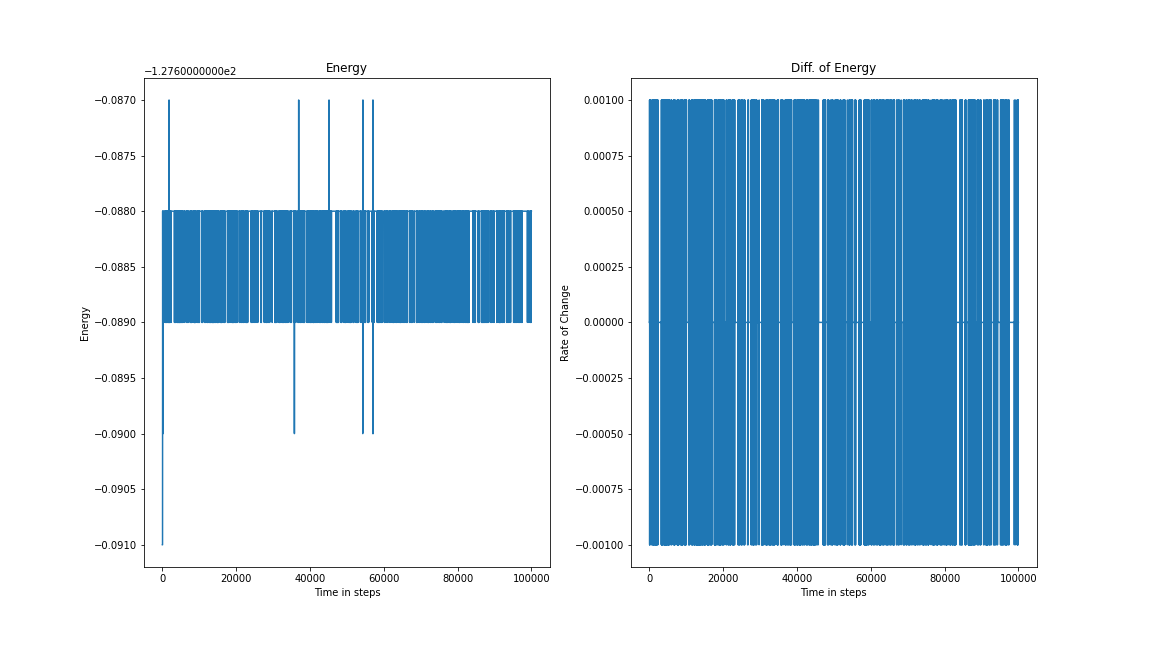
\includegraphics[scale=1]{Figure/plot_001.png}
	\end{center}
	\caption[Simulation]{Simulation with a time step of 0.001}
	\label{Plot001}
\end{figure}
\begin{figure}[!h]
	\begin{center}
		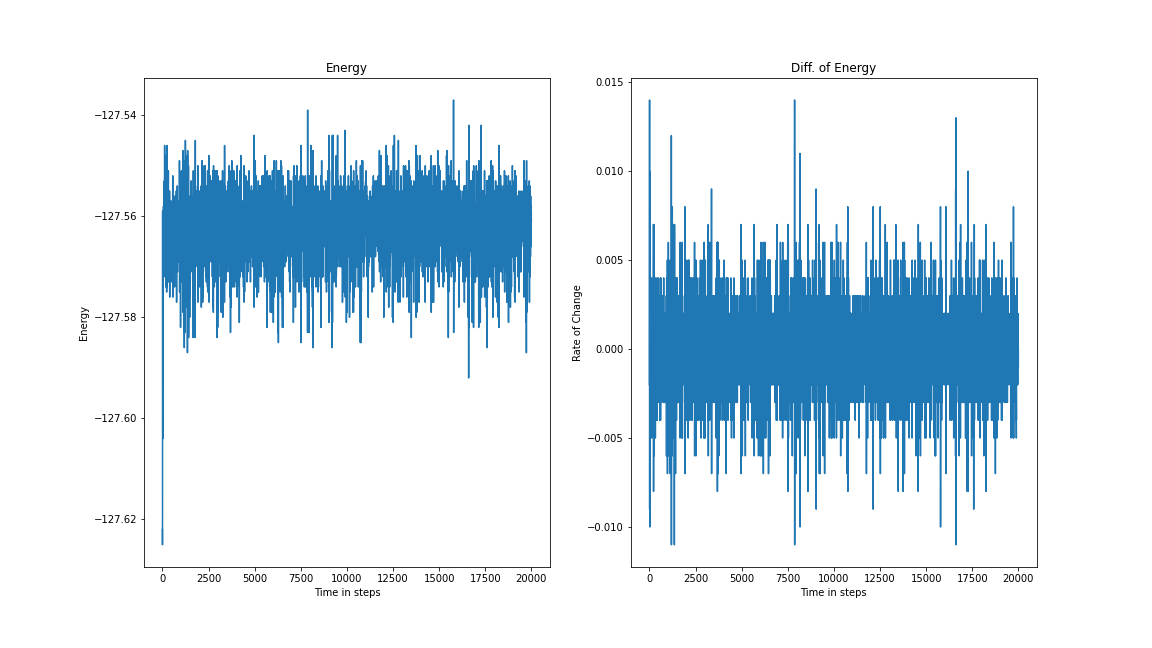
\includegraphics[scale= 1]{Figure/plot_005.png}
	\end{center}
	\caption[Simulation]{Simulation with a time step of 0.005}
	\label{Plot005}
\end{figure}
\begin{figure}[!h]
	\begin{center}
		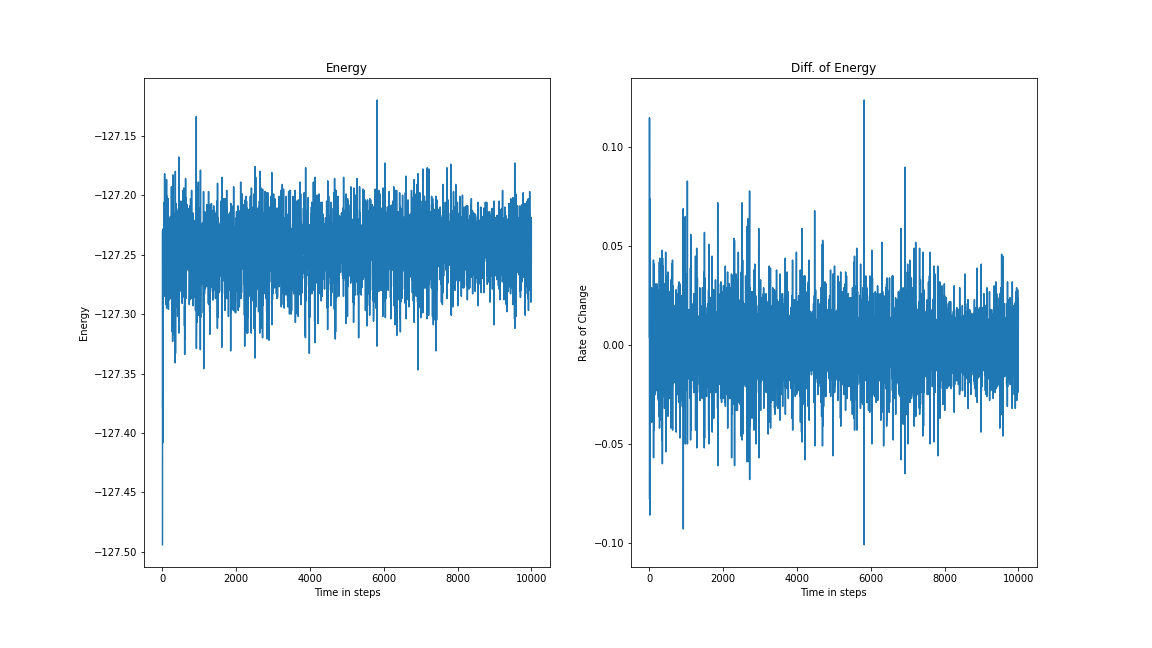
\includegraphics[scale=1]{Figure/plot_01.png}
	\end{center}
	\caption[Simulation]{Simulation with a time step of 0.01}
	\label{Plot01}
\end{figure}
\begin{figure}[!h]
	\begin{center}
		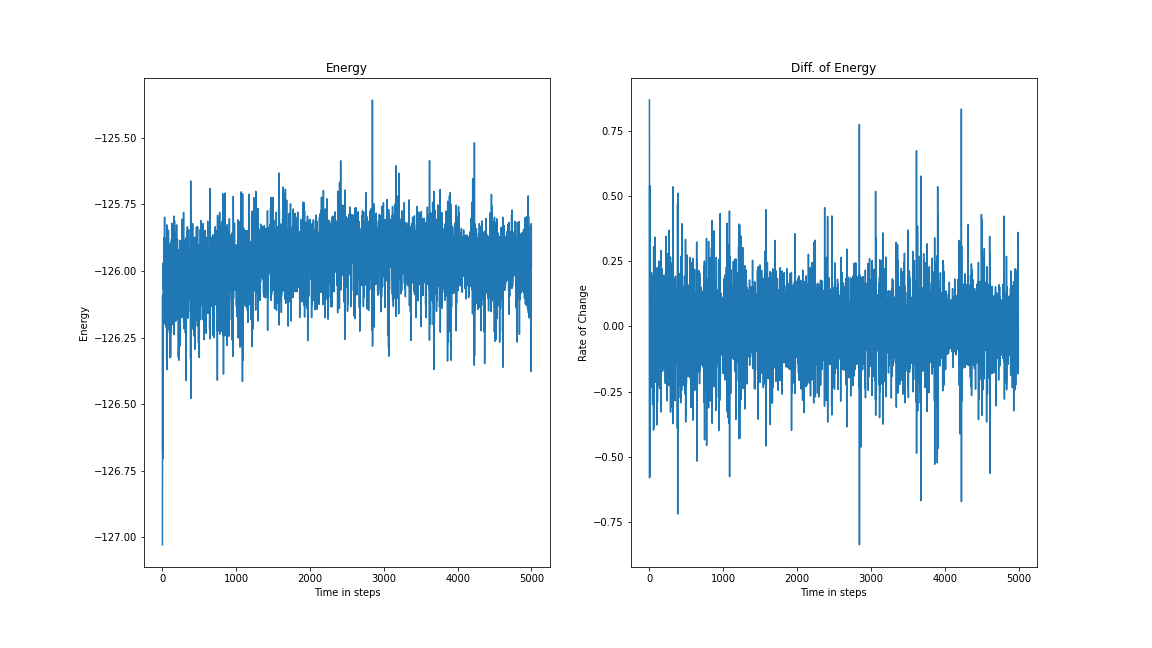
\includegraphics[scale= 1]{Figure/plot_02.png}
	\end{center}
	\caption[Simulation]{Simulation with a time step of 0.02 }
	\label{Plot02}
\end{figure}
\begin{figure}[!h]
	\begin{center}
		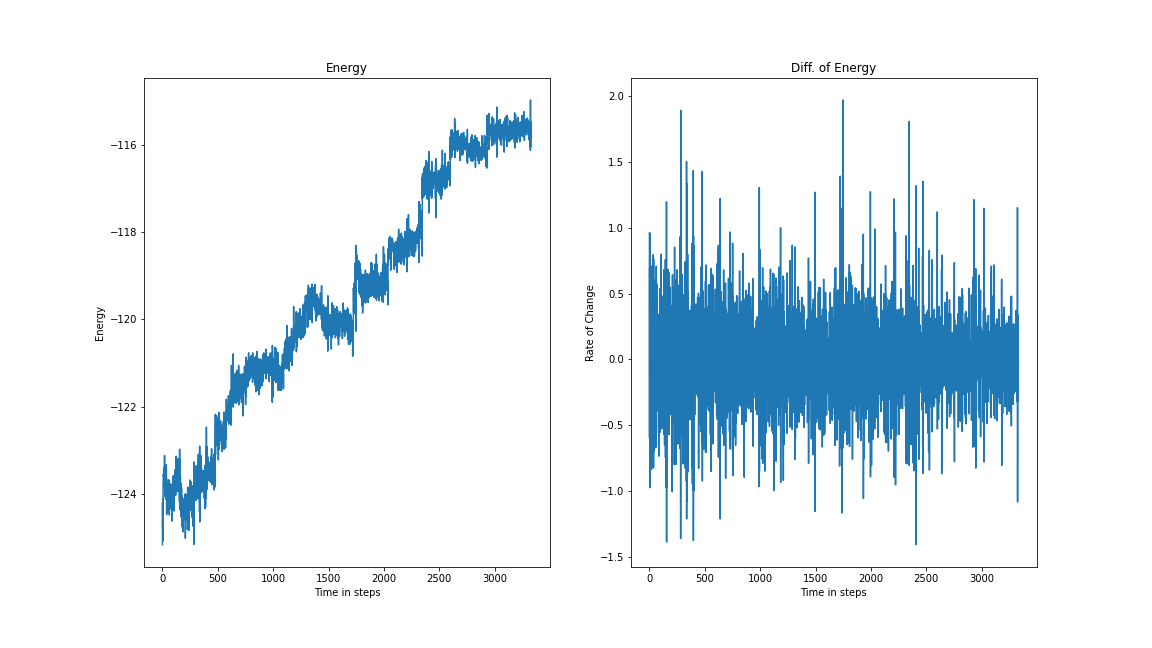
\includegraphics[scale= 1]{Figure/plot_03.png}
	\end{center}
	\caption[Simulation]{Simulation with a time step of 0.03 }
	\label{Plot03}
\end{figure}
\begin{figure}[!h]
	\begin{center}
		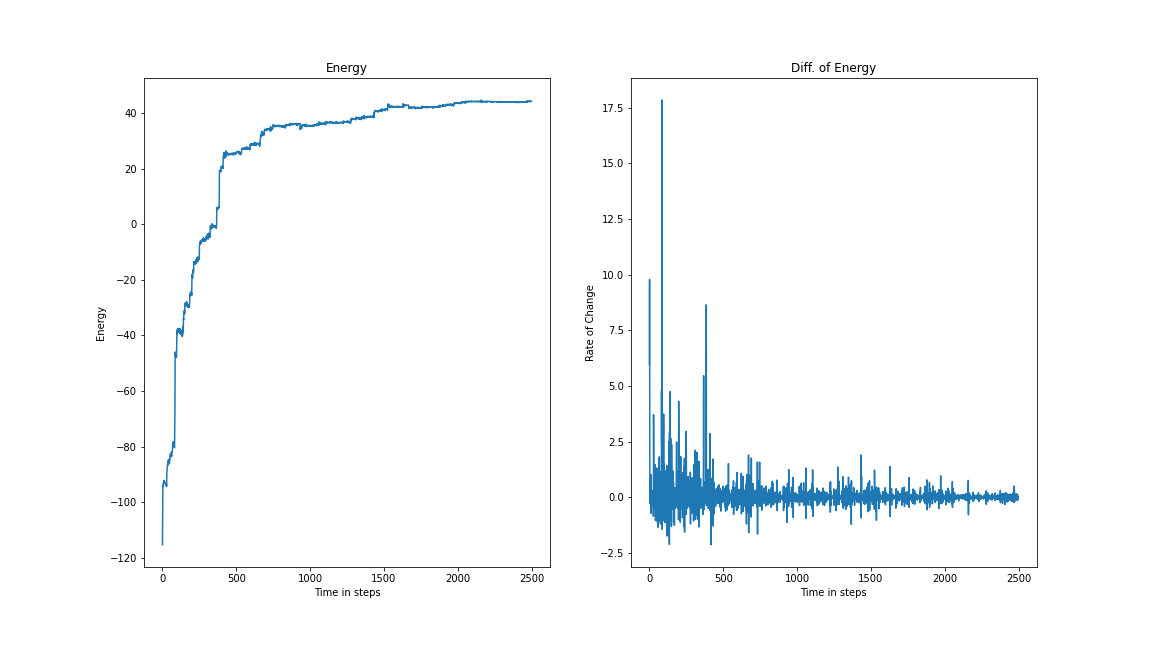
\includegraphics[scale= 1]{Figure/plot_04.png}
	\end{center}
	\caption[Simulation]{Simulation with a time step of 0.04 }
	\label{Plot04}
\end{figure}
%Snapshots of the simulation (5)
\section{Simulation Snapshots}
\begin{comment}
- not sure if i just use 2 
- background kinda bad?!
\end{comment}
\begin{figure}[!h]
	\begin{center}
		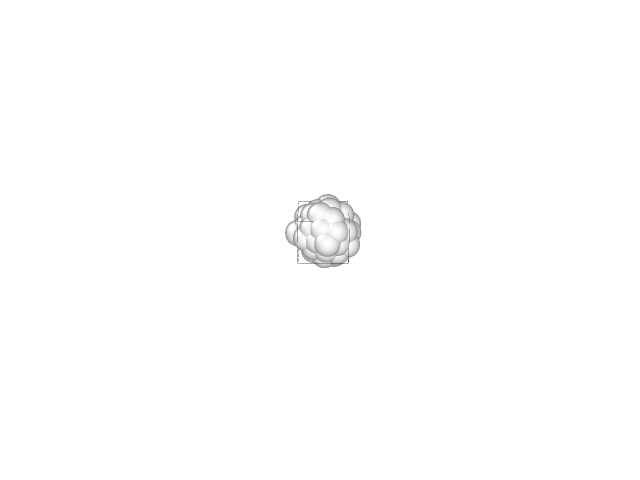
\includegraphics[scale= 1]{Figure/1Image.png}
	\end{center}
	\caption[Simulation]{Simulation }
	\label{Simulation1}
\end{figure}
\begin{figure}[!h]
	\begin{center}
		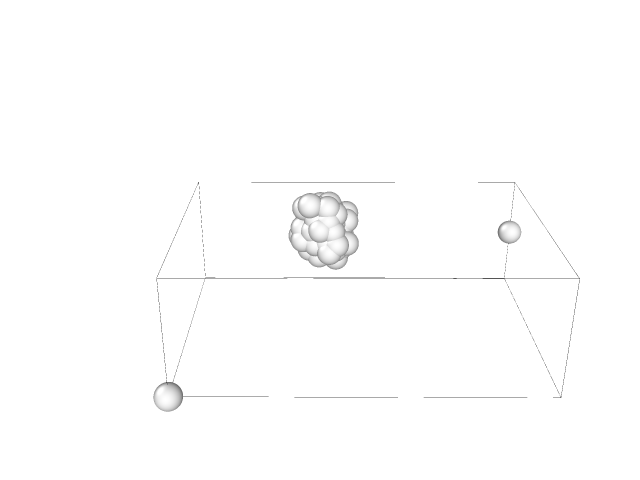
\includegraphics[scale=1]{Figure/2Image.png}
	\end{center}
	\caption[Simulation]{Simulation}
	\label{Simulation2}
\end{figure}
\begin{figure}[!h]
	\begin{center}
		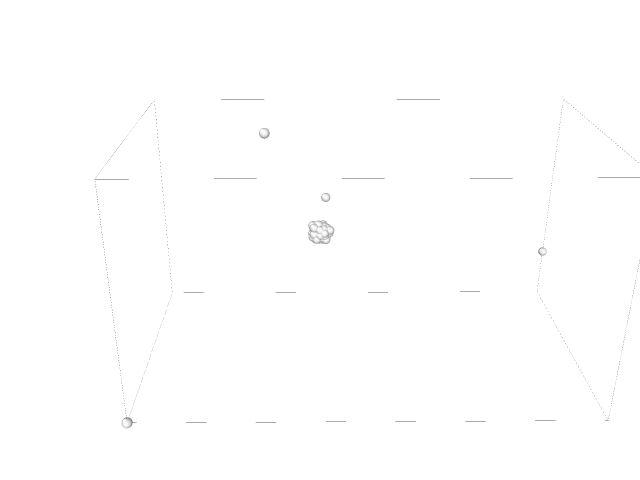
\includegraphics[scale= 1]{Figure/3Image.png}
	\end{center}
	\caption[Simulation]{Simulation }
	\label{Simulation3}
\end{figure}
\begin{figure}[!h]
	\begin{center}
		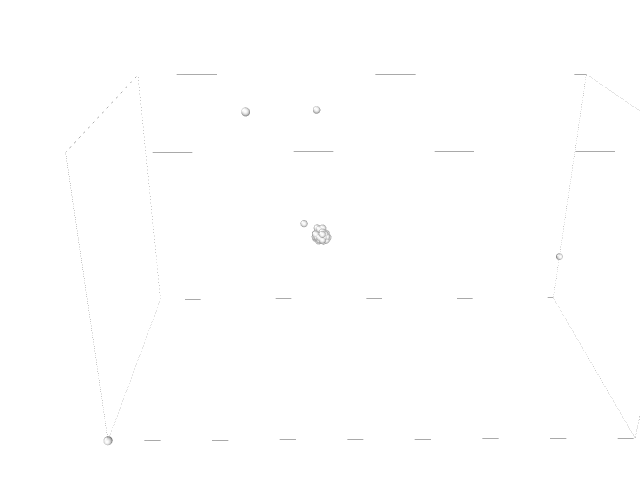
\includegraphics[scale= 1]{Figure/4Image.png}
	\end{center}
	\caption[Simulation]{Simulation }
	\label{Simulation4}
\end{figure}
\begin{figure}[!h]
	\begin{center}
		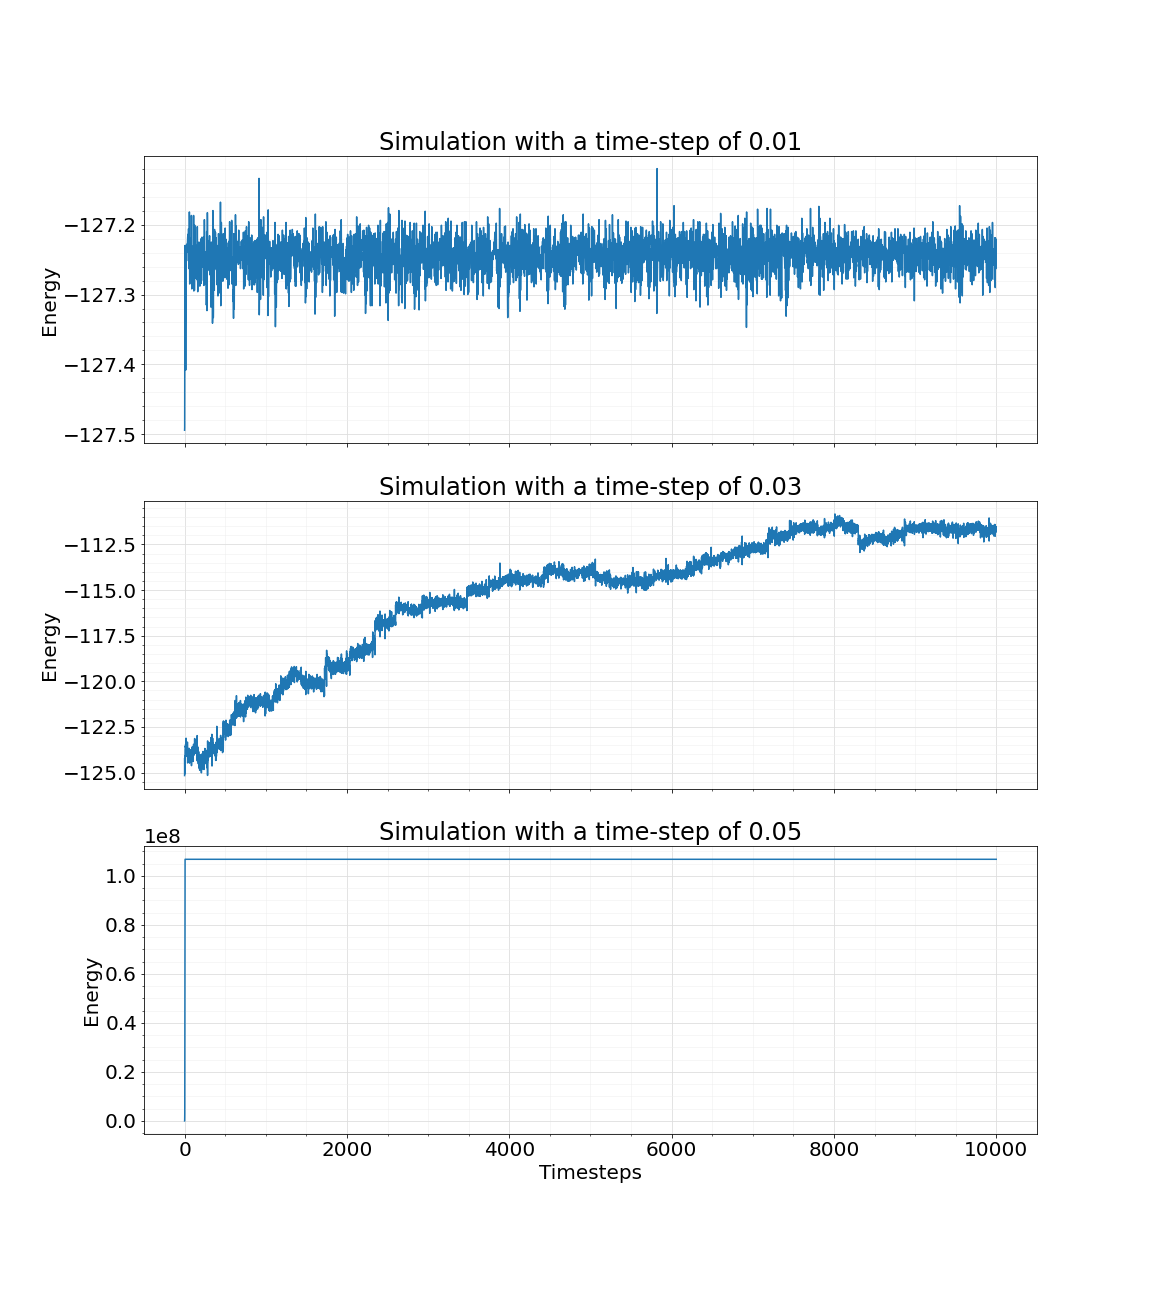
\includegraphics[scale= 1]{/home/cm/CLionProjects/MDCode/AData//totalEnergyDrift.png}
	\end{center}
	\caption[Simulation]{Simulation }
	\label{Simulation5}
\end{figure}